\documentclass[]{article}

\title{\textbf{Quantum Computation and Quantum Information}}
\author{Hsi-Sheng Goan}
\date{}

\usepackage{amsmath,amsfonts,amssymb,amsthm}
\usepackage{braket}
\usepackage[margin=1.0in]{geometry}
\usepackage{bbold}
\usepackage{enumitem}
\usepackage{mdframed}
\usepackage{ntheorem}
\usepackage{commath,mathtools}
\usepackage{dsfont}

\newtheorem*{remark}{Remark}
\newtheorem*{propos}{Proposition}
\newtheorem*{example}{Example}
\theoremstyle{nonumberplain}
\newmdtheoremenv{definition}{Definition}
\newmdtheoremenv{theorem}{Theorem}
\newmdtheoremenv{postu}{Postulate}

\begin{document}
\maketitle
\section{Overview}%
\label{sec:overview}
	53 quantum bits (Quantum supremency)\\
	Task that super computer takes 100000 years (IBM days) only takes 200 sec on Quantum Computer\\
	IBM 53 qubits have not been optimized\\
	$2^{100}$ state seems powerful \\
\section{Speech}
RSA cryptography: Factor two prime number
Factor 309-digit number: Classical THz computer take 150000 years, and quantum computer take $<$ 1s
\subsection{Quantum bit}
Classical bit: 0 or 1\\
Quantum bit: QM two-state system $\ket{\psi}=\alpha\ket{0}+\beta\ket{1}$\\
Two qubit: We can have four state simultaneously $\ket{\psi}=\alpha\ket{00}+\beta\ket{01}+\gamma\ket{10}+\tau\ket{11}$\\
So in quantum register, for 3 bit, we can have 8 states simultaneously,unlike classical register only 1 state
\subsection{Development}
2016 IBM 5-qubit online\\
2017 IBM 16-qubit online (but 1 or 2 malfunction)\\ 
50 qubits need to pay
The temperature for Quantum computer is nearly 20mK to superconduct\\
Noisy Intermediate Scale Quantum $(NISQ)$\\
In classical computer, we can prevent noise just put on threshold, but quantum error is hard to correct. We may add another error to that\\
Google v.s. IBM: 53 qubits 200s and 72 petabyte momory few days
\subsection{implementation}
\begin{itemize}
\item 1998 proposol: Sillicon-based electron-immediated nuclear spin (2012 implement)
\item  Electron spins in quantum dots
\item	2015 two-quibt logic gate in silicon (Using semiconductor 15nm!!)
\end{itemize}
\subsection{Challenge}
\begin{itemize}
	\item Much larger numbers of qubits e.g. shor's need thousand qubits
	\item	Much greater connectivity with fewer restriction
	\item Much lower error rate
	\item True fault tolerance-error correction
	\item Higher operating temperture
\end{itemize}
\subsection{HQC}
Hybrid Quantum-Classical (HQC) Algorithm\\
Variational quantum circuit algorithm\\
Data encoding scheme\\
Vairational Quantum Eigensolver (VQE)
\subsection{Application}
\begin{itemize}
	\item Artificial intelligence
	\item Medicine and Materials (Molecule simulation)
	\item Supply chain
	\item Cloud Security
\end{itemize}
\section{Quantum Computation \& Quantum Information (QC\&QI)}%
\label{sec:quantum_computation_quantum_information}
It is the study of information processing and computing tasks that can be accomplished using QM system.
\begin{remark}
IBM using classical approach to simulate 32 qubits QM system. 
\end{remark}
\begin{remark}
Quantum system is rare in our daily life. It seems the nature is against it.
\end{remark}
\begin{flushleft}
Explore and exploit Quantum effect, based on the principle of QM to compute and process information in ways that are \textbf{faster} or \textbf{more efficient} than or \textbf{even impossible} on conventional computers or information processing devices.
\end{flushleft}
\begin{example}
\ \\
Shor's Quantum factoring algorithms (1994)\\
Grover's Quantum search algorithms (1996)\\
Quantum simulation (exponential enhancement in memory size) Feynamn 1982\\
Quantum Teleportation (1993) Bennett et al.\\
Quantum superdense coding (1992)Bemett and Wiesner \\
Quantum Cryptography (1984) Bennett and Brassard
\end{example}
\begin{remark}
\textbf{Only} Quantum machine can simulate quantum system. Because quantum system grows too fast.
\end{remark}
\begin{remark}
Quantum Teleportation: Transfer quantum state from one place to another place \\
Quantum superdense coding: Use a few qubit to transfer more bit information
\end{remark}
\begin{remark}
Shor's: Prime factorization, exponential speed up\\
Grover's: Unsorted data, qudratic speed up\\ 
\end{remark}
\begin{center}
What is the killer application ?
\end{center}
\section{Quantum Information Sciences (QIS)}%
\label{sec:quantum_information_sciences}
To catch all aspectes of QC \& QI
\subsection{Fundamental questions of IS}
\begin{enumerate}
	\item \label{IS:first} Given a physical resoures - energy, time, space, bit, gates
	\item \label{IS:second} Given an information processing task - data compression, information transmission, computing task, factoring
	\item \label{IS:third} Given a criterion for success
\end{enumerate}
We ask the question: How much of \ref{IS:first} do I need to achieve \ref{IS:second} while satisfying \ref{IS:third} ?
\\
\\
Pursuing this question in the quantum case has led to and presumably will continue to lead to interesting new information processing capability.
\subsection{Knowing the rules of QM $\neq$ Understanding the QM}
\paragraph{\textbf{What high-level principles are implied by QM?}}%
\label{par:paragraph_name}
\begin{center}
	\textit{To discuss these high-level principles, we may need to know the basic rules of QM first.}\\
\end{center}
QM has a fearsome popular image because the mathematics required to apply QM to problems like determining the energy spectra of molecules and calculating scattering cross-section is difficult or intimidateing.\\
\\
By contrast, the mathematics used in application to QIS is "relatively painless". Do not need to read the tranditional QM textbooks. Here, I mean the mathematics required to understand those algorithms protocols. However, the math for physical implementation and consideration of real world, noise and decoherence may be a little bit involved.\\

\paragraph{\textbf{What is Quantum Mechanics?}}%
\label{par:paragraph_name}
\begin{center}
	\textit{Is it a complete physical therory of the world in its own right? } No!! msiconception!!\\
	It is a framework for the development of physical theory.
\end{center}

\paragraph{\textbf{QM consists of a set of mathematical postulates:\\}}%
\label{par:qm_consists_of_a_set_of_mathematical_postulates_}
\begin{center}
4 supensingly simple postulates witch lay the ground rules for our desceiption of the world.\\
\end{center}
Most physicsts believe that theory of everything will be a QM theory:
\begin{enumerate}
	\item Attempts to describe gravitation in the framework of QM has so far not yet been successful.
	\item Conceptual issue, so called "measurement problem" remains to be clarified.
\end{enumerate}
\subsection{The Structure of QM for QIS}%
\label{sec:the_structure_of_qm_for_qis}
\begin{equation*}
\begin{cases}
	\textit{linear algebra: Matrix, finite-dimension}\\
	\textit{Dirac notation:} \ket{\psi}, \bra{\phi}, \langle A \rangle\\
	\textit{4 postulates of QM}
\end{cases}
\end{equation*}
\begin{enumerate}
	\item How to describe Quantum state of a closed system? \\
		State space (Hilbert space), state vector
	\item How to describe Quantum dynamics (time evolution)? \\
		Unitary evolution
	\item How to describe measurements of a Quantum system? \\
		Projectile measurement $\rightarrow$ POVM measurement, Genernalized Quantum measurement
	\item How to describe Quantum of a composite system? \\
		tensor product
\end{enumerate}
\begin{postu}
	Associated to any isolated physical system is a complex vector space with inner product (that is Hilbert space) known as the state space of the system. Thy system is completely described by its state vector which is a unit vector in the system's state space.
\end{postu}
\begin{remark}
QM does not tell us, for a given physical system, whate the state space of that system is, nor does it tell us the state vector of the system is.
\end{remark}
\begin{remark}
	Finding that out for a specific system is a difficult problem for which physicists have developed many beautiful rules (e.g. QED)
\end{remark}
\begin{example} 
	\textbf{Quantum bit (qubit) (Two level system)}\\
"bit" is the fundamental element for information processing concept of classical Computation and Information. It can exist in two distinct states represented by 0 and 1.\\
It is over $\mathbb{C}^{2}$ and quantum state is just a unit vector in that space.
\[
\ket{\psi}=\alpha\ket{0}+\beta\ket{1}
\] 
\[
\ket{\psi} = \alpha\ket{0}+\beta\ket{1} = 
\begin{pmatrix}
\alpha \\
\beta
\end{pmatrix}_{in\  \ket{0}, \ket{1}\ basis}
= \alpha
\begin{pmatrix}
1\\
0
\end{pmatrix}
+ \beta
\begin{pmatrix}
0\\
1
\end{pmatrix}
\] 
\[
	\braket{\psi|\psi} = 
\begin{pmatrix}
	\alpha^{*} & \beta^{*}
\end{pmatrix}
\begin{pmatrix}
	\alpha\\ \beta
\end{pmatrix}
= \abs{\alpha}^{2}+\abs{\beta}^{2}=1
\] 
\end{example}
\begin{postu}
The evolution of a closed Quantum system is described by a unitary transformation
\[
	\ket{\psi(t_{2})}=U(t_{1},t_{2})\ket{\psi(t_{1})}\  \qquad\mathrlap{\textit{U is unitary to preserve normalize}}
\] 
\end{postu}
\begin{remark}
	QM does not prescribe this unitary evolution for particular system. Physicsts figure it out by a complex interplay between theory and experiement
\end{remark}
\begin{remark}
matrix = transformation = linear operator = map = Quantum gate
\end{remark}
\begin{example}
	Pauli gate (Pauli sigma matrices) \\
\[
\sigma_{x}=
\begin{pmatrix}
	0 & 1\\
	1 & 0
\end{pmatrix}
\ \sigma_{y}=
\begin{pmatrix}
	0 & -i\\
	i & 0
\end{pmatrix}
\ \sigma_{z}=
\begin{pmatrix}
	1 & 0\\
	0 & -1 
\end{pmatrix}
\ \mathds{1}=
\begin{pmatrix}
	1 & 0\\
	0 & 1 
\end{pmatrix}
\] 
\begin{figure}[!hbt]
	\centering
	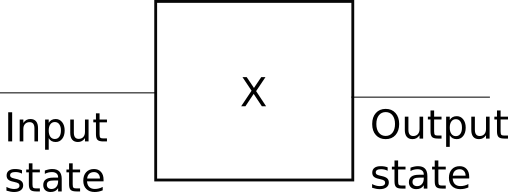
\includegraphics[scale=0.5]{1.png}
\end{figure}
\\
Quantum wire: The qubit is carried along by this Quantum wire until it reaches the X gate, not necessarily means that it carries qubit through space, may represnt a stationary qubit which is simply sitting there, passing through time until the X gate is applied.
\begin{equation*}
\begin{aligned}
	X\ket{0} &= 
\begin{pmatrix}
	0 & 1 \\
	1 & 0 
\end{pmatrix}
\begin{pmatrix}
1 \\
0
\end{pmatrix}
=
\begin{pmatrix}
0 \\
1
\end{pmatrix}
=\ket{1} 
\\
X\ket{1} &= 
\begin{pmatrix}
	0 & 1 \\
	1 & 0 
\end{pmatrix}
\begin{pmatrix}
0 \\
1
\end{pmatrix}
=
\begin{pmatrix}
1 \\
0
\end{pmatrix}
= \ket{0}
\end{aligned}
\end{equation*}
\begin{center}
Quantum NOT gate
\end{center}
\end{example}
\begin{postu}
	The time evolution of the state of a closed quantum system by Schr$\ddot{o}$dinger equation:
\[
i\hbar\frac{\partial \ket{\psi}}{\partial t} = \mathcal{H}\ket{\psi}
\] 
if $\mathcal{H}$ is independent of time
\[
	U(t_{1},t_{2}) = e^{-i\mathcal{H}(t_{2}-t_{1})/\hbar}
\] 
if $\mathcal{H}$ depends on time, we have to do the integration on Hamiltonian
\end{postu}
\begin{postu}[General Measurement]
	Quantum measurements are described by a collection $\{M_{n}\}$ of measurement operators. There are operators acting on the state space of the system being measured. The index m refers to the measurement outcomes that may occur in the experiment. If the state of the quantum system is $\ket{\psi}$ immediately before the measurement then:
\begin{enumerate}
	\item The probability that result m occurs is given by 
		\[
			p(m) = \braket{\psi|M_{m}^{\dagger}M_{m}|\psi}
		\] 
	\item And the state of the system after the measurement is 
		\[
			\frac{M_{m}\ket{\psi}}{\sqrt{\braket{\psi|M_{m}^{\dagger}M_{m}|\psi}}}
		\] 
\end{enumerate}
The measurement operators satisfy the completeness equation $\sum^{}_{m} M^{\dagger}_{m}M_{m}=\mathds{1}$ 
\end{postu}
\begin{example}
\textbf{Measurement of a qubit in the computation basis}
\begin{equation*}
\begin{aligned}
	\ket{\psi} &= \alpha\ket{0}+\beta\ket{1}\\
				  &=	\frac{1}{\sqrt{2}}[(\alpha+\beta)\ket{+}+(\alpha-\beta)\ket{-}] \\
\end{aligned}
\end{equation*}
\begin{equation*}
\begin{aligned}
	M_{0} &= \ket{0}\bra{0}=M_{0}^{\dagger} \\
	M_{1} &= \ket{1}\bra{1}=M_{1}^{\dagger}
\end{aligned}
\end{equation*}
\begin{itemize}
	\item Probability
		\[
			p(0) = \braket{\psi|M_{0}^{\dagger}M_{0}|\psi} = \braket{\psi|M_{0}|\psi} = \abs{\alpha}^{2}
		\] 
		\[
			p(1) = \braket{\psi|M_{1}^{\dagger}M_{1}|\psi} = \braket{\psi|M_{1}|\psi} = \abs{\beta}^{2}
		\] 
	\item Post-Measurement
\[
	\frac{M_{m}\ket{\psi}}{\sqrt{\braket{\psi|M_{m}^{\dagger}M_{m}|\psi}}}=\frac{\alpha}{\sqrt{\abs{\alpha}^{2}}}\ket{0}=\frac{\alpha}{\abs{\alpha}^{2}}\ket{0}=e^{i\theta}\ket{0}
\] 
\end{itemize}
\end{example}
\begin{remark}
\[
\mathcal{O}=
\begin{pmatrix}
	\mathcal{O}_{00} & \mathcal{O}_{01} \\
	\mathcal{O}_{10} & \mathcal{O}_{11} \\
\end{pmatrix}
\ and \ 
\mathcal{O} = \sum^{}_{i,j} \mathcal{O}_{ij}\ket{i}\bra{j}
\] 
\end{remark}
\begin{remark}
Global phase doesn't matter, but relative phase does.
\end{remark}
\newpage
\paragraph{Bloch Shpere representation}%
\ \\
\begin{figure}[!hbt]
\centering
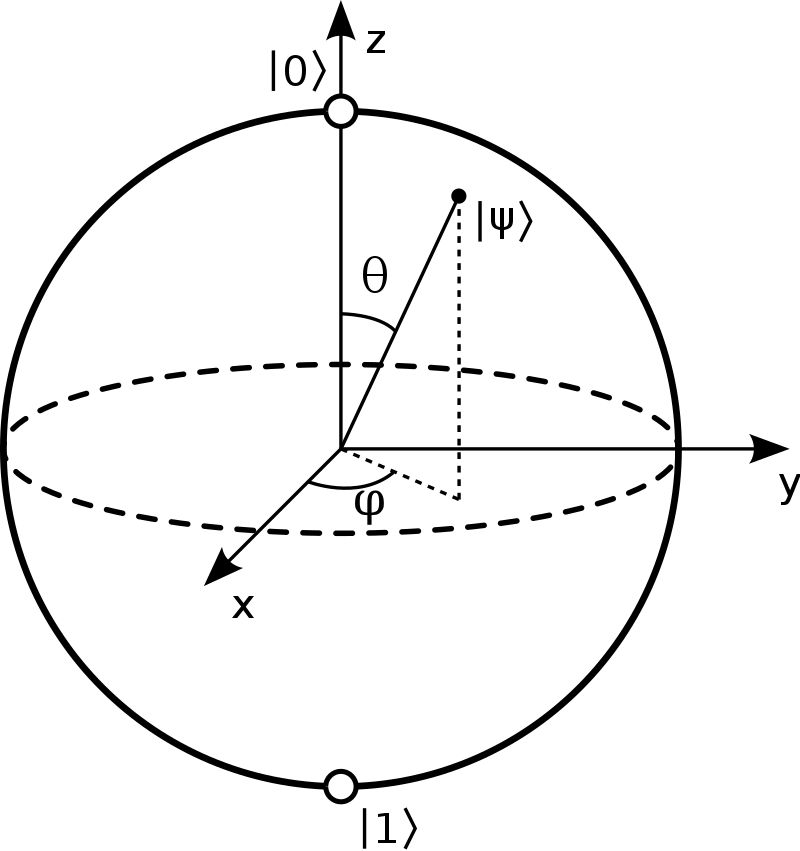
\includegraphics[scale=0.1]{2.png}
\end{figure}
\begin{equation*}
\begin{aligned}
	& \hat{n}=(\sin{\theta}\cos{\phi},\sin{\theta}\sin{\phi},\cos{\phi})\\
	& \ket{+}_{\hat{n}}=\cos{\frac{\theta}{2}}\ket{0}+e^{i\phi}\sin{\frac{\theta}{2}} \ket{1} \\
	& \ket{-}_{\hat{n}}=-\sin{\frac{\theta}{2}}\ket{0}+\cos{\frac{\theta}{2}} e^{i\phi}\ket{1}
\end{aligned}
\end{equation*}
$\ket{+}_{n}$ means the eigenstate of Pauli matrix in $\hat{n}$ direction. That is, $\hat{\sigma} \cdot \hat{n}$. \\
For arbitrary state, the expectation value $\braket{X}^{2}+\braket{Y}^{2}+\braket{Z}^{2}=1$
\begin{remark}
	In Quantum Mechanics, we can not determined all spin component simultaneously since $[S_{i},S_{j}]=i\hbar\epsilon_{ijk}S_{k}$. Hence, in quantum case, we can only calculate the expectation value of three obervables $S_{x},S_{y},S_{z}$.
\end{remark}
\begin{remark}
\\
\[
	\textit{qubit: } \ket{\psi} = \cos{\frac{\theta}{2}}\ket{0}+\sin{\frac{\theta}{2}}e^{i\phi}\ket{0}
\] 
Since $\theta$ and $\phi$ are continuous, it seems that we can carry all information in $\theta$ and $\phi$. However, if we want to extract the probability of $\ket{0}$, we have to prepare "many" pure state. But the precision of the coefficient is related to how many pure state we observe. If we can do measurement infinitely, then we can get exact qunit.  
\end{remark}
\paragraph{Distinguishing Quantum States}%
\label{par:paragraph_name}
\ \\
\\
Distinguishibility: a set of states $\ket{\psi_{i}}$, $1 \leq i \leq n$ known to Alice and Bob. Alice choose a state $\ket{\psi_{i}}$ and gives it to Bob, whose task is to identify the index j of the state Alice has given him.
\begin{enumerate}
	\item Suppose $\ket{\psi_{i}}$ are orthonormal $\braket{\psi_{i}|\psi_{j}}=\delta_{ij}$. Define $M_{j}=\ket{\psi_{j}}\bra{\psi_{j}}$. If the state $\ket{\psi_{j}}$ is prepared, then $p(j)=\braket{\psi_{j}|M_{j}^{\dagger}M_{j}|\psi_{j}}=1$ ; $p(i)=\braket{\psi_{i}|M_{j}^{\dagger}M_{j}|\psi_{i}}=0$. 
\begin{remark}
	Since Alice only choose n states, there are some states that are not chosen. Hence, we adjust the completness relation $ \sum^{n}_{i=1} M_{i}^{\dagger}M_{i} + M_{0}^{\dagger}M_{0}=\mathbb{1}$. $M_{0}$ is the rest of the states.
\end{remark}
	\item If the state $\ket{\psi_{i}}$ are not orthonormal then there is no Quantum measurement capable of distinguishing these state. $\braket{\psi_{i}|\psi_{j}}\neq 0$ for $i\neq j$
\end{enumerate}
\begin{postu}[Projective measurement]
A projective measurement is described by an observable, a Hermitian operator $\mathcal{M}$ with spectral decomposition
\[
\mathcal{M}= \sum^{}_{m} m P_{m}
\] 
where $P_{m}=\ket{m}\bra{m}$ is the projector onto the eigenspace of $\mathcal{M}$ with eigenvalue m. \\ \\
The possible outcomes of the measurement correspond to the eigenvalues m and the outcome m occurs with probability
\[
	p(m)=\braket{\psi|P_{m}|\psi}
\] 
The corresponding post-measurement is 
\[
	\frac{P_{m}\ket{\psi}}{\sqrt{\braket{\psi|P_{m}|\psi}}}
\] 
\end{postu}
\begin{example}
\[
S_{z}=
\frac{\hbar}{2}\ket{+}\bra{+} - \frac{\hbar}{2}\ket{-}\bra{-} 
\] 
\end{example}
\begin{remark}
Projective measurement can be usderstood as a special case of general  measurement
\[
	\sum^{}_{m} M^{\dagger}_{m}M_{m}=\mathbb{1}
\] 
From postulate of projective measurement, $M_{m}^{\dagger}=M_{m} (Hermition)$ and $M_{m}M_{m'}=M_{m}\delta_{mm'} (Orthogonal Projector)$  $p(m) = \braket{\psi|M^{\dagger}_{m}M_{m}|\psi}=\braket{\psi|M_{m}|\psi}$ and $\frac{M_{m}\ket{\psi}}{\sqrt{\braket{\psi|M^{\dagger}_{m}M_{m}|\psi}}}=\frac{M_{m}\ket{\psi}}{\sqrt{p(m)}}=\frac{M_{m}\ket{\psi}}{\sqrt{\braket{\psi|M_{m}|\psi}}}$
\end{remark}
\paragraph{The Heisenberg uncertainty principle}%
\label{par:the_heisenberg_uncertainty_principle}
\ \\
\\
Suppose A and B are two Hermitian operators $A^{\dagger}=A, B^{\dagger}=B$. Suppose $\braket{\psi|AB|\psi}=x+iy$ where $x,y \in \mathbb{R}$ 
\[
\braket{\psi|BA|\psi}=\braket{\psi|B^{\dagger}A|\psi}=\braket{\psi|A^{\dagger}B|\psi}^{*}=\braket{\psi|AB|\psi}^{*}
\] 
\[
	\braket{\psi|[A,B]|\psi}=\braket{\psi|AB-BA|\psi}=2iy
\] 
\[
	\braket{\psi|\{A,B\}|\psi}=\braket{\psi|AB+BA|\psi}=2x
\] 
\[
	\abs{\braket{\psi|[A,B]|\psi}}^{2}+\abs{\braket{\psi|\{A,B\}|\psi}}^{2}=4\abs{\braket{\psi|AB|\psi}}^{2}
\] 
By the Cauchy-Schwartz inequality:
\[
\abs{\braket{\psi|AB|\psi}}^{2} \leq \braket{\psi|A^{2}|\psi}\braket{\psi|B^{2}|\psi}
\] 
Hence
\[
	\abs{\braket{\psi|[A,B]|\psi}}^{2}\leq 4\abs{\braket{\psi|AB|\psi}}^{2}\leq 4\braket{\psi|A^{2}|\psi}\braket{\psi|B^{2}|\psi}
\] 
Suppose C and D are two obervables and $A=C-\braket{C}, B=D-\braket{D}$$\Rightarrow [A,B]=[C,D]$
\[
	\abs{\braket{\psi|[C,D]|\psi}}^{2} \leq 4(\Delta C)^{2}(\Delta D)^{2}
\] 
\[
	\frac{1}{2}\abs{\braket{\psi|[C,D]|\psi}}\leq (\Delta C)(\Delta D)
\] 
There is an intrinsic limit to the accureacy of the simultaneous measurement of both C and D if $[C,D]\neq 0.$ \\
The measurement of one observable necessarily disturbs the other if $[C,D]\neq 0$
\paragraph{Positive Operator-valued Measure (POVM) measurement}%
\label{par:paragraph_name}
\ \\
\\
\textbf{Positive operator:} A special subclass of Hermitian operators defined as for any vector $\ket{v}, \braket{v|A|v}$ is a real, non-negative numbers.\\
\\
\textbf{Positive definite:} If $\braket{v|A|v}$ is strictly greater than zero for all $\ket{v}\neq 0$\\
\\
\textbf{POVM:} A set of $\{E_{m}\}, \sum^{}_{m} E_{m}=\mathbb{1}, p(m)=\braket{\psi|E_{m}|\psi}$
\begin{remark}
	POVM is a simple consequence of the general measurement. The set of $E_{m}$ is sufficient to determine probabilriy of different outcomes m. The complete set $\{E_{m}\}$ is known as POVM. $E_{m}$ is the POVM element.
\end{remark}
\begin{example}
\begin{equation*}
\begin{aligned}
	\ket{{\psi_{1}}}&=\ket{0}\\
	\ket{\psi_{2}}&=\frac{\ket{0}+\ket{1}}{\sqrt{2}}
\end{aligned}
\end{equation*}
It is impossible for Bob to perform a measurement which distinguishes the states. \\
Consider POVM containing 
\begin{equation*}
\begin{aligned}
	E_{1}&=\frac{\sqrt{2}}{1+\sqrt{2}}\ket{1}\bra{1}\\
	E_{2}&=\frac{\sqrt{2}}{1+\sqrt{2}}\frac{(\ket{0}-\ket{1})(\bra{0}-\ket{1})}{2}\\
	E_{3}&=\mathbb{1}-E_{1}-E_{2}
\end{aligned}
\end{equation*}
If the outcome is $m_{1}$, the state will not be $\ket{\psi_{1}}$ since $\braket{\psi_{1}|E_{1}|\psi_{1}}=0$. The state must be $\ket{\psi_{2}}$.\\
If the outcome is $m_{2}$, the state will not be $\ket{\psi_{2}}$ since $\braket{\psi_{2}|E_{2}|\psi_{2}}=0$. The state must be $\ket{\psi_{1}}$.\\
If the outcome is $m_{3}$, however, we do not sure whether we get $\ket{\psi_{1}}$ or $\ket{\psi_{2}}$. We get no information.
\end{example}
\end{document}
